\chapter{Implementierungen}
\label{chap_impl}

Den Inhalt des folgenden Kapitels bilden die im Rahmen dieser Arbeit verwendeten bzw. selbsterstellten Implementierungen. So wird zunächst die verwendete Implementierung des Lernalgorithmus präsentiert, da sich aus ihr Folgeanforderungen für die Implementierung der Neural Map sowie der Umgebungen für die Experimente ergeben. Darüber hinaus werden die Hyperparameter des Algorithmus vorgestellt. Im Anschluss daran wird die selbsterstellte Implementierung der Neural Map erörtert. Hierbei liegt der Fokus insbesondere auf den Implementierungsdetails der Operatoren. Danach wird die im Rahmen dieser Arbeit erdachte Erweiterung des Schreiboperators ausführlich erklärt. Sie bildet zusammen mit der ursprünglichen Variante der Neural Map den Hauptgegenstand der im weiteren Verlauf durchgeführten Experimente.


\section{OpenAI Baseline und OpenAI Gym}
\label{ppo_impl}

Da der Fokus dieser Arbeit nicht auf einer Untersuchung des Lernalgorithmus liegt, wird auf eine bereits bestehende Implementierung zurückgegriffen. Das Unternehmen OpenAI, dessen Schwerpunkt auf der Forschung im Bereich künstlicher Intelligenz liegt, hat die Open Source Reinforcement Learning Bibliothek OpenAI Baseline entwickelt \cite{Baselines}. Dabei lag der Fokus darauf, Forschung im Bereich Reinforcement Learning vergleichbarer zu machen und das Entstehen neuer Ideen zu begünstigen. Zu diesem Zweck enthält die Bibliothek eine Vielzahl von fertig implementierten und umfangreich getesteten Lernalgorithmen, unter anderen auch eine Version des PPO Algorithmus. Außerdem verfügt sie über einige Modelle zur Parametrisierung der Policy bzw. State-Value Funktion. Insbesondere enthält sie auch eine Implementierung eines LSTM, wie es in Abschnitt \ref{sec_lstm} beschrieben wurde. Dieses soll in den Experimenten als Referenz für die verschiedenen Varianten der Neural Map dienen. Somit enthält OpenAI Baseline bis auf entsprechende Umgebungen, mit denen die Lernalgorithmen ein Modell trainieren können, alle zum Reinforcement Learning benötigten Komponenten. An dieser Stelle kommt dann die aus dem gleichen Hause stammende Bibliothek OpenAI Gym ins Spiel. Zum einen sind in ihr verschiedenste Umgebungen enthalten, die die Möglichkeit für Benchmarks unterschiedlichster Art bieten. Zum anderen definiert die Bibliothek auch die am weitesten verbreitete Schnittstelle für Reinforcement Learning Umgebungen. Diese ermöglicht es Lernalgorithmen und Umgebungen komplett getrennt voneinander und zugleich möglichst generisch zu entwickeln. Auch in dieser Arbeit werden die Umgebungen unter Berücksichtigung der OpenAI Gym Schnittstelle erstellt. Dies geschieht schon alleine aus dem Grund, dass die benutzte PPO Implementierung eine Umgebung mit der entsprechenden Schnittstelle erwartet.

Die OpenAI Baseline Implementierung des PPO Algorithmus entspricht im Wesentlichen den in Abschnitt \ref{sec_ppo} vorgestellten Grundlagen. Insbesondere greift die Implementierung zur Durchführung der benötigten Berechnungen auf Tensorflow in der API Version 1 zurück. Dies wiederum ermöglicht es, die Ausführung des Algorithmus auf eine Grafikkarte auszulagern. Da die im Reinforcement Learning Kontext verwendeten Modelle oftmals Neuronale Netze verschiedenster Gestalt sind, lässt sich auf diese Art in der Regel die benötigte Trainingszeit reduzieren. Die Ursache hierfür liegt in der Fähigkeit von Grafikkarten, eine Vielzahl von Berechnungen parallel ausführen zu können. Die Berechnungen, die beim Training Neuronaler Netze anfallen, lassen sich wiederum sehr gut parallellisieren. Für diese Arbeit ist relevant, dass das im weiteren Verlauf präsentierte Modell der Neural Map auch in Tensorflow implementiert werden muss. Grundsätzlich verwendet die Implementierung des PPO Algorithmus zwei Modelle. Das eine Modell wird als Act-Model bezeichnet und das andere als Train-Model. Das Act-Model wird zur Interaktion mit der Umgebung verwendet, d.h. es generiert Schritt für Schritt die Trainingsdaten, indem es auf Basis des Zustands die Aktionen auswählt und die State-Value Funktion schätzt. Dieser Vorgang wird solange wiederholt, bis der Batch von Trainingsdaten die gewünschte Größe erreicht hat. Anschließend wird das Train-Modell mit diesen Daten trainiert. Dazu wird unter Berücksichtigung der Verlustfunktion ein Gradientenschritt zur Anpassung der Modell-Parameter getätigt. Dieser Vorgang wiederholt sich wechselseitig, bis eine bestimmte Anzahl an Trainingsschritten erreicht wird. Da während des Trainings nur die Parameter des Train-Model angepasst werden und Tensorflow Modelle darüber hinaus ohne eine Veränderung ihrer Struktur beliebige Batch-Größen verarbeiten können, kann für die beiden zuvor beschriebenen Modelle dasselbe Tensorflow-Modell in der Implementierung verwendet werden. Auf diese Weise bewirkt das Training des Train-Model auch ein besseres Verhalten des Act-Model. Dies führt zu besseren Trainingsdaten und verbessert somit das Training des Train-Model. Dieses Wechselspiel entspricht dem Actor-Critic Ansatz. Im folgenden sollen die Hyperparameter vorgestellt werden, die das Verhalten des Algorithmus im Detail steuern und darüber hinaus auch Verwendung in den Experimenten finden.

\begin{description}
	\item • nsteps: Dieser Parameter gibt an, über wie viele Schritte das Act-Modell Daten sammelt. Er entspricht somit der Batch-Größe beim Training des Train-Modells.
	\item • total\_timesteps: Die Gesamtanzahl im Rahmen des Trainings getätigter Schritte, d.h. in der Umgebung ausgeführte Aktionen, wird über diesen Parameter spezifiziert. Außerdem ergibt sich aus der ganzzahligen Division von total\_timesteps durch nsteps, die Anzahl an Trainingsupdates.
	\item • ent\_coef: Hierbei handelt es sich um den Entropie Koeffizienten $c_2$ aus der Verlustfunktion (vgl. Gleichung \eqref{L_gesamt}).
	\item • lr: Die Lernrate wird über diesen Parameter angegeben.
	\item • vf\_coef: Dies ist der Koeffizient $c_1$ aus der Verlustfunktion (vgl. Gleichung \eqref{L_gesamt}) zur Gewichtung des auf der geschätzten State-Value Funktion basierenden Verlustterms.
	\item • max\_grad\_norm: Die Implementierung schneidet den Gradienten ab, wenn dessen Norm größer ist als der Wert dieses Parameters. Somit wird wie durch die abgeschnittene Verlustfunktion auch auf Implementierungsebene ein zu großes Update der Policy bzw. State-Value Funktion verhindert.
	\item • gamma: Hierbei handelt es sich um den Discount Faktor (vgl. Gleichung \eqref{return_eq}).
	\item • noptepochs: Dieser Parameter gibt an, für wie viele Trainingschritte bzw. Paramter-Updates ein Batch von Daten genutzt wird.
	\item • cliprange: Das Epsilon aus der  geclippten Verlustfunktion (vgl. Gleichung \eqref{L_CLIP}) wird durch diesen Parameter spezifiziert.
\end{description}



Die OpenAI Gym Schnittstelle für Reinforcement Learning Umgebungen wurde ebenfalls von OpenAI entworfen und folgt dem Paradigma der objektorientierten Programmierung \cite{Gym}. Die wichtigsten Attribute der resultierenden Klasse sind der observation\_space und der action\_space. Diese erteilen Auskunft über die Form des Zustandsraums und des Aktionsraums. Sie geben beispielsweise an, aus wie vielen Pixeln ein Zustand besteht oder wie viele Aktionen in einer Umgebung möglich sind. Innerhalb der PPO Implementierung werden sie verwendet, um das Tensorflow-Modell korrekt anzulegen, d.h. um die Gestalt des Eingangs (Zustand) und des Ausgangs (Aktion) zu berücksichtigen. Die wichtigsten beiden Methoden sind zum einen die reset Methode und zum anderen die step Methode. Erstere setzt die Umgebung in ihren Anfangszustand zurück. Dieser kann entweder fix sein, also immer gleich, oder zufällig. Die Methode wird zu Beginn jeder Episode aufgerufen. Der Rückgabewert der Methode besteht aus dem Anfangszustand $s_0$. Die step Methode wird verwendet, um einen Interaktionsschritt mit der Umgebung zu vollziehen. Dazu bekommt sie als Eingabe eine Aktion $a_t$ übergeben. Als Rückgabe liefert die Methode wie erwartet den Reward $R_{t+1}$ und den Folgezustand $s_{t+1}$. Darüber hinaus gibt sie eine boolsche Variable mit dem Namen done zurück. Deren Wert ist true, wenn der letzte Schritt die Umgebung in einen Terminalzustand versetzt hat und false andernfalls. Somit kannder Lernalgorithmus anhand dieser Variablen den Aufruf der reset Methode gesteuert werden.


\section{Implementierung der Neural Map}
\label{sec_nm_impl}

Wie bereits im vorangegangenen Abschnitt erörtert, erfolgt die im Rahmen dieser Arbeit erstellte Implementierung der Neural Map aus Kompatibilitätsgründen in Tensorflow. Dazu werden die Gleichungen aus Abschnitt \ref{sec_neural_map} in entsprechende Funktionen der Tensorflow Bibliothek übersetzt.

Die Größe des internen Speichers der Neural Map $M$ wird aus dem Paper übernommen und beträgt $32 \times 15 \times 15$. Da die vertikale und horizontale Größe 15 beträgt, ergben sich somit 225 Speicherpositionen an den jeweils ein 32-dimensionales Feature gespeichert ist.

Die Global Read Operation besteht aus einem Neuronalen Faltungsnetz. Die Parameter dieses Netzes können aus dem Paper übernommen werden. Somit besteht es aus drei Faltungsschichten und zwei Fully Connected Schichten. Die Faltungsschichten enthalten jeweils 8 Filter der Größe $3 \times 3$. Der Stride beträgt 2 in der ersten Schicht und 1 in den beiden weiteren Schichten. In der ersten Schicht findet ein Padding mittels Nullen statt, in den beiden Weiteren nicht. Die erste Fully Connected Schicht enthält 256 Neuronen, die andere enthält als Resultät der Feature-Dimension $C$ des internen Speichers 32 Neuronen. Als Aktivierungsfunktion wird in allen Schichten die relu-Funktion verwendet, außer in der letzten Schicht kommt $tanh$ zum Einsatz.

Die Context Read Operation enthält keine frei wählbaren Hyperparameter. Die einzigen trainierbaren Parameter sind in der Gewichtsmatrix $W$ enthalten und deren Zeilen- und Spaltenanzahl kann direkt aus der zugrunde liegenden Vektor-Matrix-Gleichung bestimmt werden, also aus der Größe des Zustands und der Feature-Dimension $C$ des internen Speichers.

Zu den weiteren Neuronalen Netzen der Neural Map finden sich keinerlei Details innerhalb des Papers. Somit wird ihre Struktur vom Verfasser dieser Arbeit festgelegt. Das Netz der Local Write Operation besteht aus drei Fully Connected Schichten, wovon die ersten beiden über 256 Neuronen verfügen und die Letzte wieder über 32. Als Aktivierungsfunktion wird in den ersten beiden Schichten die relu-Funktion verwendet, in der Letzten $tanh$. Das finale Neuronale Netz verfügt zwei Fully Connected Schichten, die beide 256 Neuronen besitzen und die relu-Funktion als Aktivierungsfunktion haben. Eine weitere Schicht zur Prädiktion der Aktionen muss nicht explizit hinzugefügt werden. Diese Aufgabe übernimmt das OpenAI Baseline Paket, welches dem Modell zum einen eine weitere Schicht zur Prädiktion der Aktionen anhängt. Hierbei wird selbstverständlich der Aktionsraum der Umgebung berücksichtigt. Parallel dazu wird dem Modell noch eine weitere Schicht hinzugefügt, um die State-Value Funktion zu schätzen. Somit wird die Ausgabe der letzten Schicht des finalen Netzes sowohl in eine Schicht zur Aktionsauswahl gegeben, als auch in eine zur Schätung der State-Value Funktion, d.h. es kann dasselbe Modell für beide Aufgaben verwendet werden.

Die Update Operation entspricht aus Implementierungssicht einer selektiven Wertzuweisung. Diese wird von Tensorflow nicht unterstützt und würde auch keinerlei Vorteile hinsichtlich der Ausführung auf einer Grafikkarte mit sich bringen, da es sich bei ihr um keine Berechnung handelt, sondern um einen einfachen Speicherzugriff. Somit ist die Update Operation nicht Teil des Tensorflow Modells, sondern wird im Anschluss außerhalb durchgeführt. Das Tensorflow Modell generiert lediglich den dafür benötigten Write Vektor. Dieser wird dann an die entsprechende Position des internen Speichers geschrieben. Der so aktualisierte Speicher wird dann im nächsten Schritt wieder als Eingabe an das Tensorflow Modell übergeben. Ähnliches gilt für das Feature an der aktuellen Position $M_t^{(x_t,y_t)}$, das für die Berechnung der Write Operation benötigt wird. Auch dieses wird vorab aus dem internen Speicher $M$ extrahiert und dann als seperate Eingabe an das Tensorflow Modell übergeben. Insgesamt ergibt sich somit, dass der interne Speicher $M$ außerhalb des Tensorflow Modells verwaltet wird.

\subsection{Erweiterung der Neural Map für 3D-Umgebungen}
\label{sec_nm_3d_ext}

Zum Umgang mit 3D-Umgebungen haben die Autoren des Papers eine Erweiterung für die Neural Map vorgestellt. Da der Zustand einer 3D-Umgebung für gewöhnlich aus einem Bild besteht, wird dieses zuerst mit einem Neuronalen Faltungsnetz prozessiert. Die Ausgabe dieses Faltungsnetzes geht dann anstelle des ursprünglichen Zustands $s_t$ in die in Abschnitt \ref{sec_neural_map} beschriebenen Operatoren bzw. Gleichungen ein. Das hierfür verwendete Faltungsnetz besteht zunächst aus einer Faltungsschicht mit 32 Filtern der Größe $8 \times 8$ und einem Stride von 4. Diese wird gefolgt von einer weiteren Faltungsschicht mit 64 Filtern der Größe $4 \times 4$ und einem Stride von 2. Abschließend kommt eine Fully Connected Schicht mit 512 Neuronen. In den Faltungsschichten wird die relu-Funktion als Aktivierungsfunktion verwendet, in der Fully Connected Schicht $tanh$.


\section{Erweiterung des Schreiboperators der Neural Map}
\label{sec_write_ext}

Bei der im Rahmen dieser Arbeit entwickelten Erweiterung des Schreiboperators ist folgende Überlegung von zentraler Bedeutung. Der ursprüngliche Schreiboperator hat nur für die aktuelle Position des Agenten $(x_t,y_t)$ ein Feature generiert und damit anschließend auch nur den internen Speicher an dieser Position, also $M_t^{(x_t,y_t)}$, aktualisiert. Da sich die Wahrnehmung eines Agenten in einer 2- bzw. 3-dimensionalen Umgebung jedoch fast nie nur auf seine aktuelle Position beschränkt, ist eine naheliegende Überlegung, ob aus dieser Wahrnehmung nicht auch noch Informationen extrahiert werden können, die eine sinnvolle Generierung eines weiteren Features zur Aktualisierung des internen Speichers ermöglichen. Analog zur menschlichen Wahrnehmung stellt für gewöhnlich die Blickrichtung des Agenten die Richtung dar, in der die aktuelle Wahrnehmung die meisten Informationen über die Umgebung enthält. Somit bildet die Blickrichtung die Grundlage für die Erweiterung des Schreiboperators, da basierend auf ihr die nächste Speicherposition bestimmt wird, für die ein weiteres Feature berechnet wird. Anschließend wird die entsprechende Position mit dem Feature aktualisiert. Somit werden pro Berechnungsschnitt der Neural Map zwei Speicherpositionen des internen Speichers $M$ aktualisiert. Der Gedanke dabei ist, dass auf diese Weise die Umgebung des Agenten hoffentlich schneller im internen Speicher der Neural Map abgebildet werden. Dies wiederum könnte zum einen in einer schnelleren Erkundung der Umgebung münden und zum anderen könnten sich durch die Erweiterung des Schreiboperators die Wahrscheinlichkeit erhöhen, dass relevante Informationen der Umgebung auch ihren Weg in den internen Speicher finden.

Der erweiterte Schreiboperator wird im Folgenden als $write_{ext}(\dots)$ bezeichnet und beschreibt die Speicherposition $(x_{ext_t},y_{ext_t})$. Das dazu verwendete Feature wird in Analogie zu dem bereits bestehenden Schreiboperator mit $w_{t+1}^{(x_{ext_t},y_{ext_t})}$ gekennzeichnet. In den 2-dimensionalen Gitterwelten, die im weiteren Verlauf dieser Arbeit als Umgebungen für die Experimente genutzt werden, existieren vier Blickrichtungen. Diese werden mit oben, unten, links und rechts bezeichnet. Die nächste Speicherposition in Blickrichtung ergibt sich dann, indem wahlweise der $x$- oder $y$-Wert der aktuellen Position um Eins verringert oder erhöht wird. Somit lässt sich die nächste Position in Blickrichtung $(x_{ext_t},y_{ext_t})$ berechnen als:

\begin{equation}
\begin{aligned}
(x_{ext_t}, y_{ext_t}) =
\begin{cases}
(x_t + 1,y_t), & \quad \text{für Blichrichtung nach rechts} \\
(x_t,y_t + 1), & \quad \text{für Blichrichtung nach unten} \\
(x_t - 1,y_t), & \quad \text{für Blichrichtung nach links} \\
(x_t,y_t - 1), & \quad \text{für Blichrichtung nach oben}
\end{cases}
\end{aligned}
\end{equation}

Diese bestimmt nicht nur die Position, an die das zusätzlich generierte Feature geschrieben wird, sondern auch die Speicherposition, von der das aktuelle Feature als Eingabe für den erweiterten Schreiboperator verwendet wird. Dieses Feature stellt den einzigen Unterschied dar im Bezug auf die Eingabe des erweiterten Schreiboperators im Vergleich zum bereits Bestehenden. Somit besteht die weitere Eingabe für den erweiterten Schreiboperator aus dem aktuellen Zustand $s_t$, dem aktuellen Global Read Vektor $r_t$ und dem aktuellen Contex Read Vektor $c_t$.
Diese Eingabe wird wie bei dem bereits vorhandenen Schreiboperator von einem Neuronalen Netz verarbeitet. Das dazu verwendete Netz verfügt über dieselbe Struktur wie das der bestehenden Schreiboperation. Das von ihm generierte Feature $w_{t+1}^{(x_{ext_t},y_{ext_t})}$ wird zum einen als zusätzliche Eingabe des finalen Netzes verwendet und zum anderen für die Update Operation. Somit wird es auch zur Aktualisierung des internen Seichers $M_t$ genutzt und folglich erweitert sich auch die Definition der Update Operation wie folgt:

\begin{equation}
 \begin{aligned}
 M_{t+1}^{(a,b)} =
 \begin{cases}
 w_{t+1}^{(x_t,y_t)}, & \quad \text{für} (a,b) = (x_t,y_t) \\
 w_{t+1}^{(x_{ext_t},y_{ext_t})}, & \quad \text{für} (a,b) = (x_{ext_t},y_{ext_t}) \\
 M_t^{(a,b)}, & \quad \text{sonst}
 \end{cases}
 \end{aligned}
\end{equation}

Die Abbildung \ref{fig_neural_map_extW} zeigt die Neural Map mit der Erweiterung des Schreiboperators. Auf der linken Seite befinden sich wieder die Eingaben $s_t$ und $M_t$ für den Zeitschritt $t$. Die Features $M_t^{(x_t,y_t)}$ und $M_t^{(x_{ext_t},y_{ext_t})}$ können wieder aus $M_t$ extrahiert werden und bilden auf diese Weise eigenständige Eingaben. Sowohl das Map Update als auch das finale Neuronale Netz erhalten als zusätliche Eingabe den Schreibvektor der erweiterten Schreiboperation (Local Write Ext) $w_{t+1}^{(x_{ext_t},y_{ext_t})}$. Darüber hinaus wird die Ausgabe des finalen Neuronalen Netzes wie in Abschnitt \ref{ppo_impl} beschrieben in zwei weitere Fully Connected Schichten gegeben. Davon erzeugt die Eine die Policy $\pi(a|s)$ und die Andere die State-Value Funktion $V(s)$. Beide werden zur Berechnung der Verlustfunktion aus Gleichung \ref{L_gesamt} benötigt.


\begin{figure}[ht!]
  \centering
  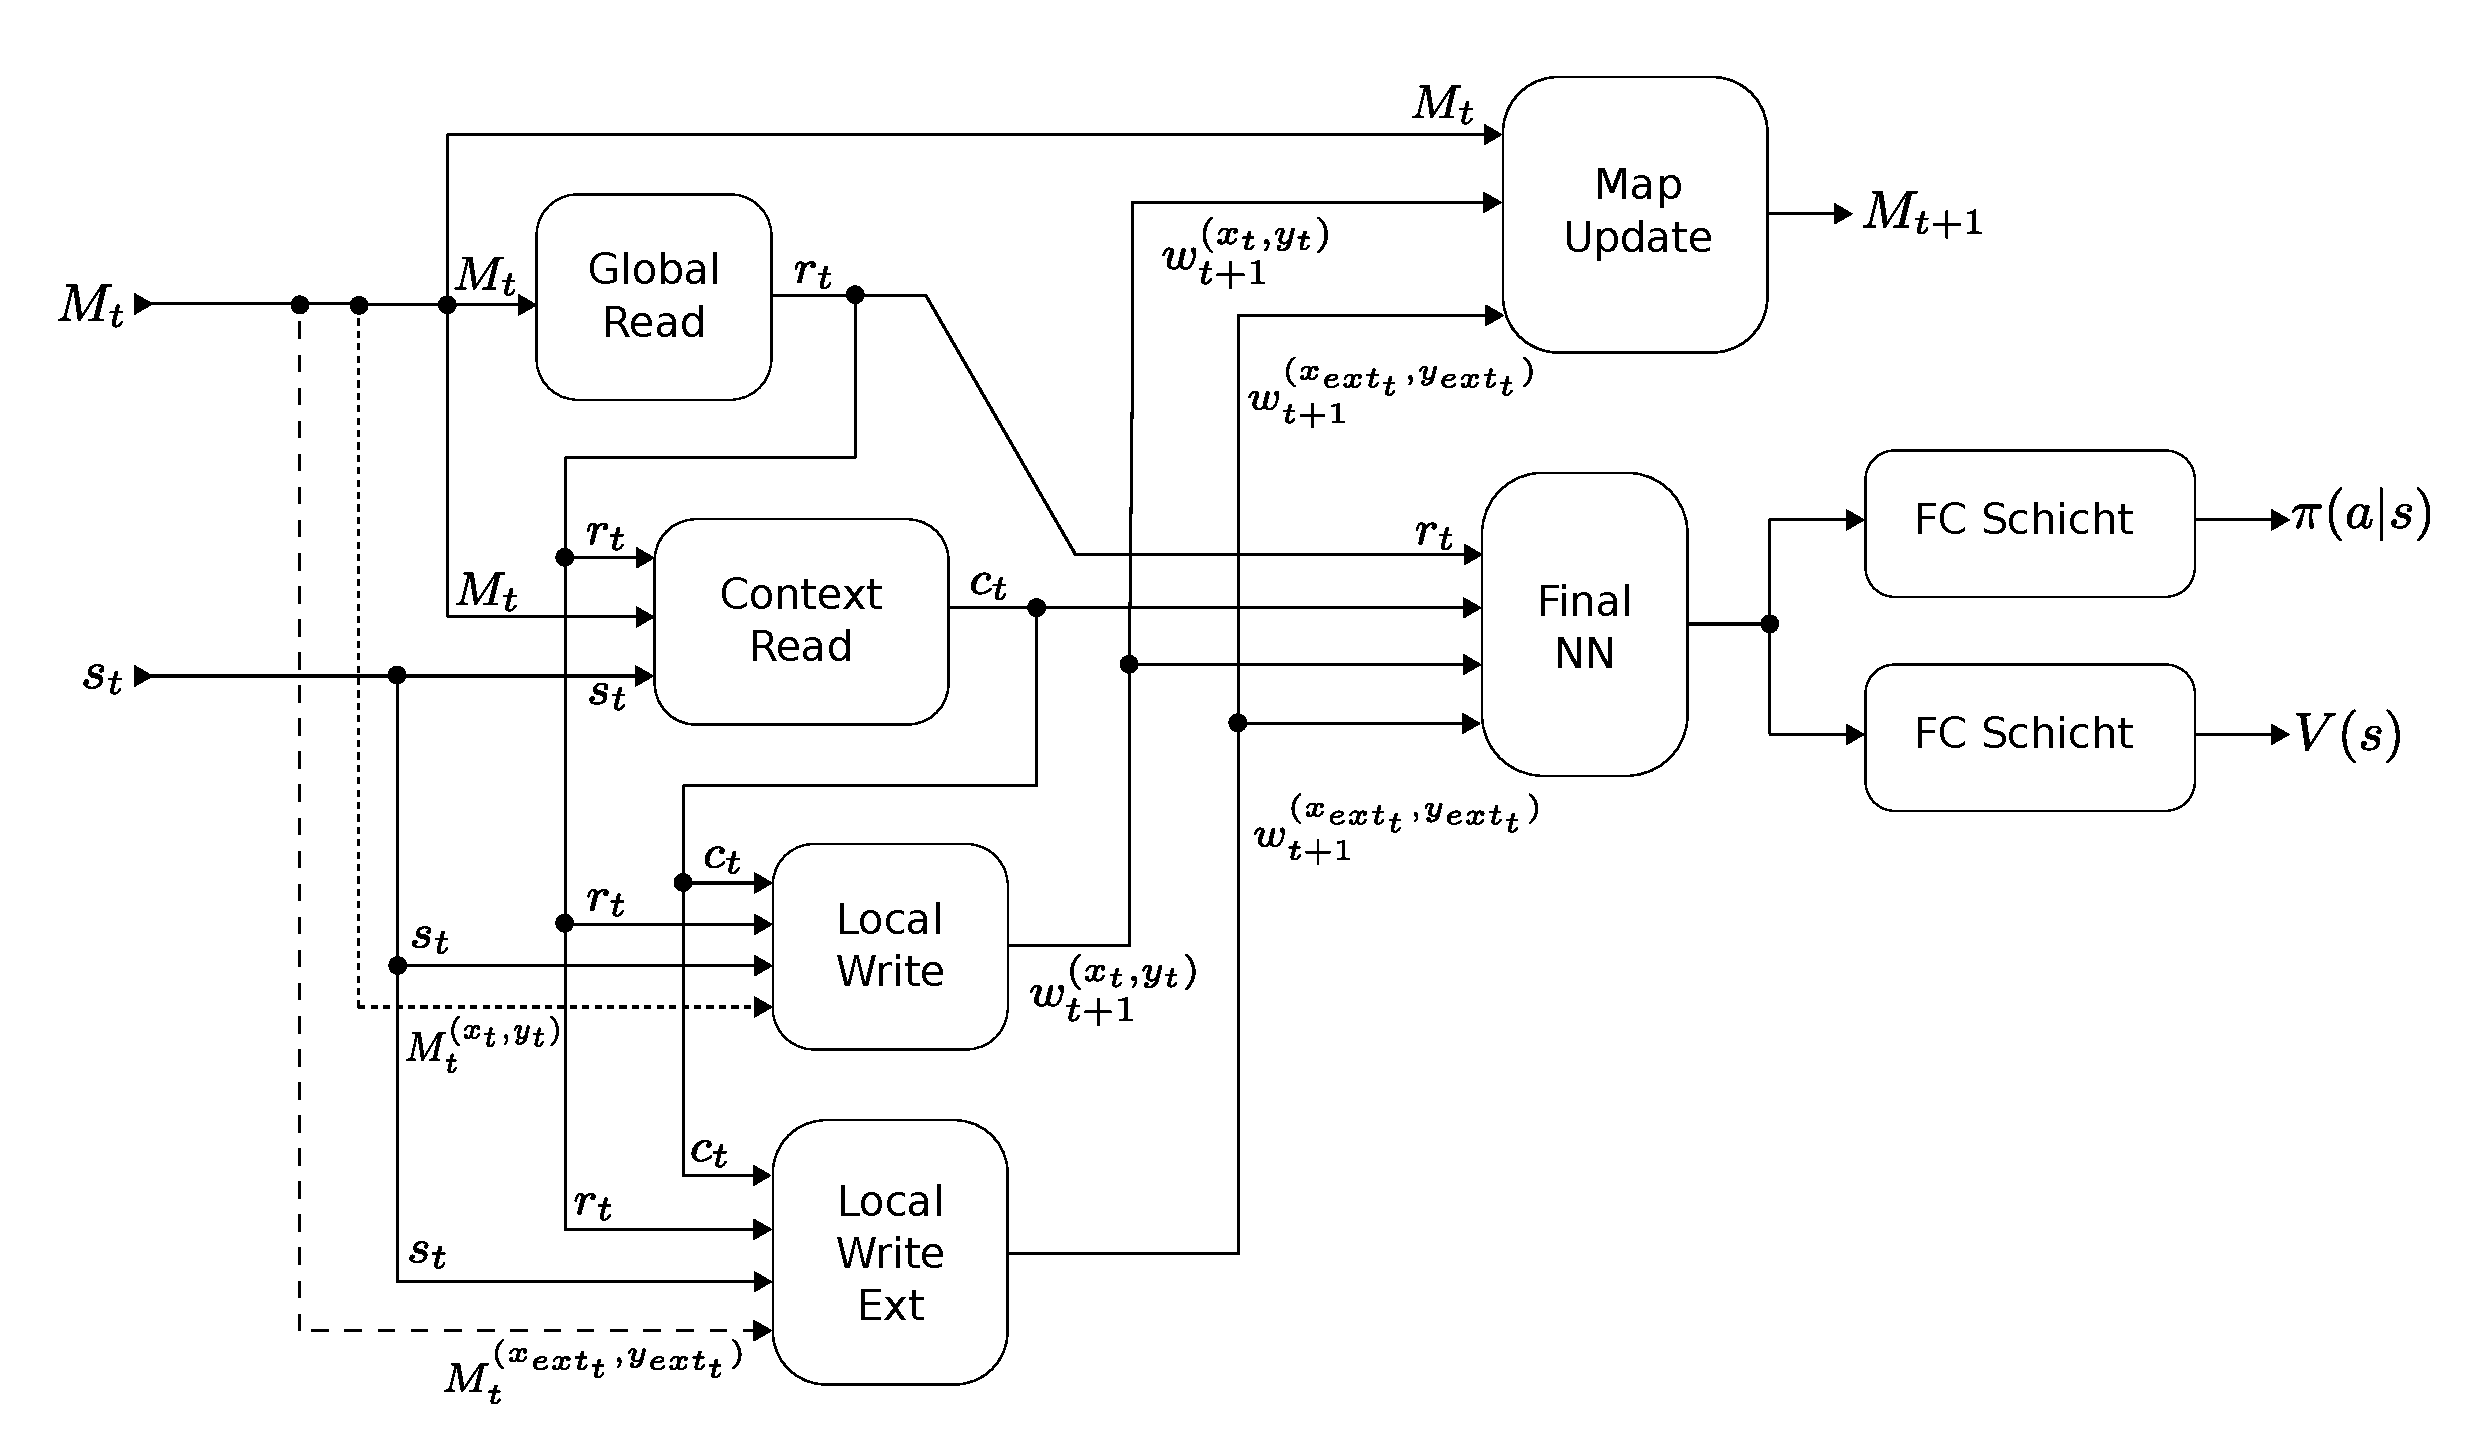
\includegraphics[keepaspectratio,width=1.0\textwidth]{abbildungen/neural_map_extW.pdf}
  %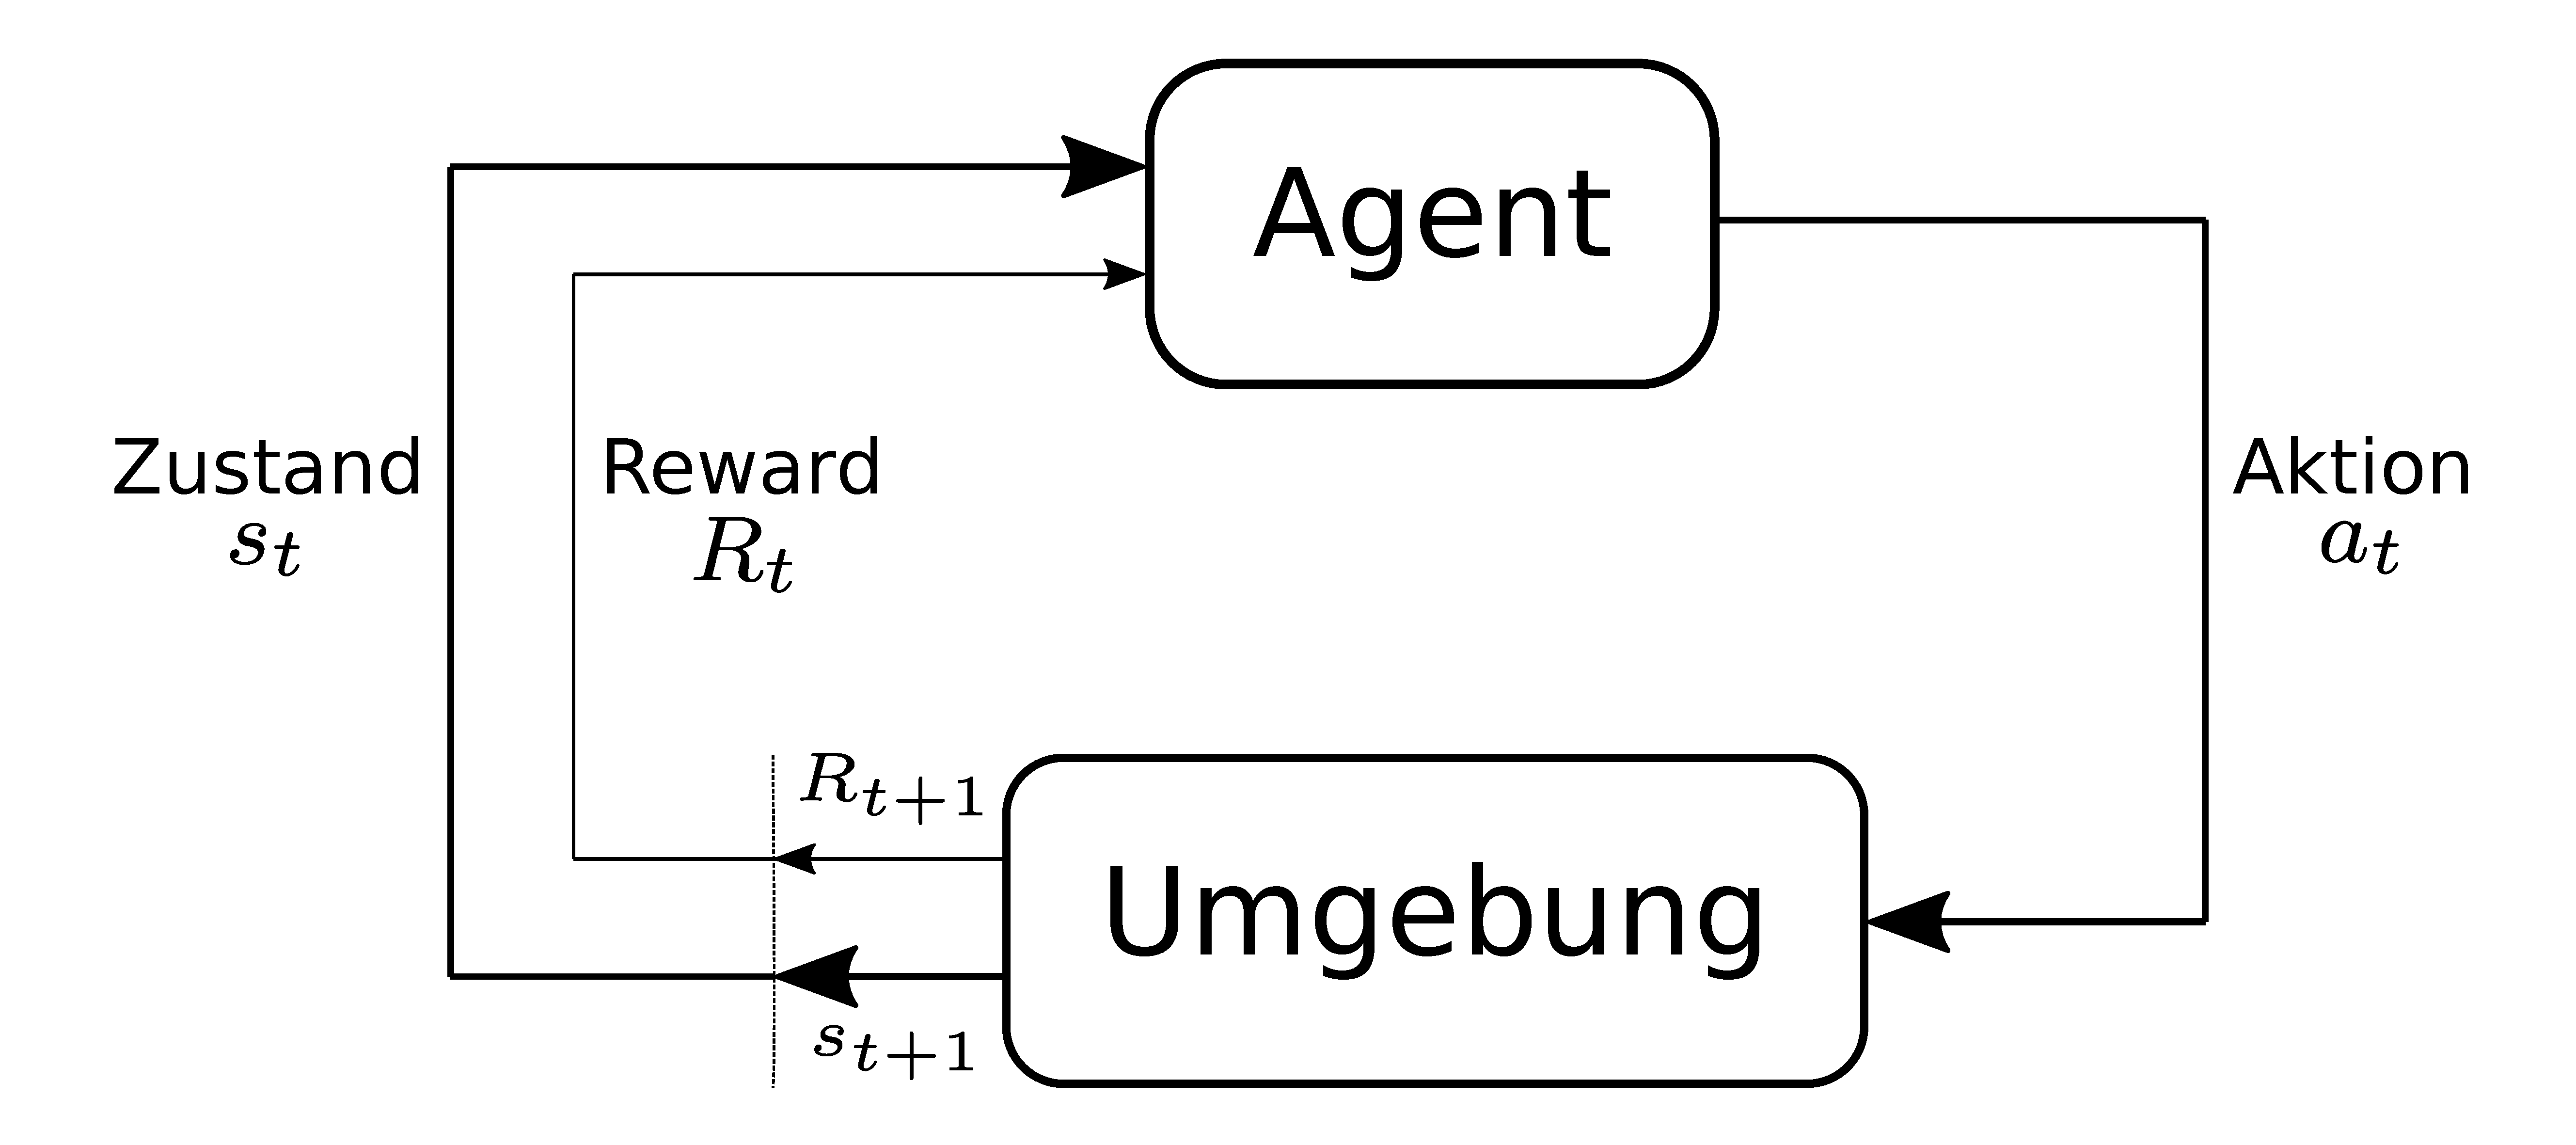
\includegraphics[height=0.5\textwidth, width=0.9\textwidth]{abbildungen/schnittstelle_agent_umgebung.pdf}
  \caption{Die Abbildung zeigt die Neural Map mit der Erweiterung des Schreiboperators (Local Write Ext). Dieser erhält im Unterschied zum bereits vorhandenen Schreiboperator als Eingabe das Feature $M_t^{(x_{ext_t},y_{ext_t})}$ und generiert wiederum das Feature $w_{t+1}^{(x_{ext_t},y_{ext_t})}$. Dieses wird als zusätzliche Eingabe für die Update Operation und das finale Neuronale Netz verwendet. Darüber hinaus sind die beiden zusätzlichen Fully Connected Schichten dargestellt, die auf Basis der Ausgabe des finalen Neuronalen Netzes die Schätzung der Policy $\pi(a|s)$ und der State-Value Funktion $V(s)$ übernehmen.}
  \label{fig_neural_map_extW}
\end{figure}
